\documentclass{beamer}
\usepackage[latin1]{inputenc}
%\usetheme{Warsaw}             % Themes are listed here: https://latex-beamer.com/tutorials/beamer-themes/ 
\usetheme{Madrid}
\usepackage{multirow}
\usepackage{listings}
\definecolor{links}{HTML}{2A1B81}
\hypersetup{colorlinks,linkcolor=,urlcolor=links}
\newcommand{\CC}{\texttt{C}\nolinebreak\hspace{-.05em}\raisebox{.4ex}{\tiny\bf +}\nolinebreak\hspace{-.10em}\raisebox{.4ex}{\tiny\bf +}}
\newcommand{\quotes}[1]{``#1''}

\AtBeginSection[]{
  \begin{frame}
  \vfill
  \centering
  \begin{beamercolorbox}[sep=8pt,center,shadow=true,rounded=true]{title}
    \usebeamerfont{title}\insertsectionhead\par%
  \end{beamercolorbox}
  \vfill
  \end{frame}
}

\definecolor{BrickRed}{rgb}{0.8,0.25,0.33}
\definecolor{ForestGreen}{rgb}{0.13,0.55,0.13}
\definecolor{RoyalBlue}{rgb}{0.25,0.41,0.88}

\lstdefinestyle{MyCudaStyle}{
  %backgroundcolor=\color{white},
  basicstyle=\small\ttfamily,
  %breakatwhitespace=false,
  %breaklines=true,
  morekeywords={None},
  captionpos=b,
  commentstyle=\color{RoyalBlue},   % comment style
  frame=single,
  keywordstyle=\color{ForestGreen}\bfseries,      % keyword style
  language=C,
  showstringspaces=false,
  stringstyle=\color{BrickRed},
  emph={%
        cudaFree, cudaMalloc, cudaError\_t, cudaSuccess, 
	size\_t,
	cudaMemcpy, cudaMemcpyKind,
	cudaMemcpyHostToHost, cudaMemcpyHostToDevice, 
	cudaMemcpyDeviceToHost, cudaMemcpyDeviceToDevice,
	\_\_global\_\_, \_\_device\_\_ ,\_\_host\_\_,<<<,>>>,
	\_\_constant\_\_,
	dim3,\_\_shared\_\_,\_\_syncthreads,
	uint3,gridDim,blockIdx,blockDim, 
	threadIdx.x,threadIdx.y,threadIdx.z,threadIdx,
        cudaGetDeviceCount,cudaGetDeviceProperties,cudaDeviceProp, 
	%
        }, emphstyle={\color{ForestGreen}\bfseries}
}

\title{Introduction to GPU Programming}
%\subtitle{}
\author{Wim R.M. Cardoen}
\institute{Center of High-Performance Computing (CHPC) \\ University of Utah}
\date{October 14, 2024}

\begin{document}        % Begin Document

% --- PRELUDE ---
\begin{frame}           % Title Page
\titlepage
\end{frame}
         % Title
\begin{frame}           % Table of Contents
\frametitle{Outline}
\tableofcontents
\end{frame}
       % Table of Contents - Outline

% --- BODY ---
\section{Motivation}   % Motivation

\begin{frame}
  \frametitle{Theoretical GFLOP/s: GPU vs. CPU}	
  \begin{columns}
  \column{0.9\textwidth}
    \begin{figure}[H]
       \centering
            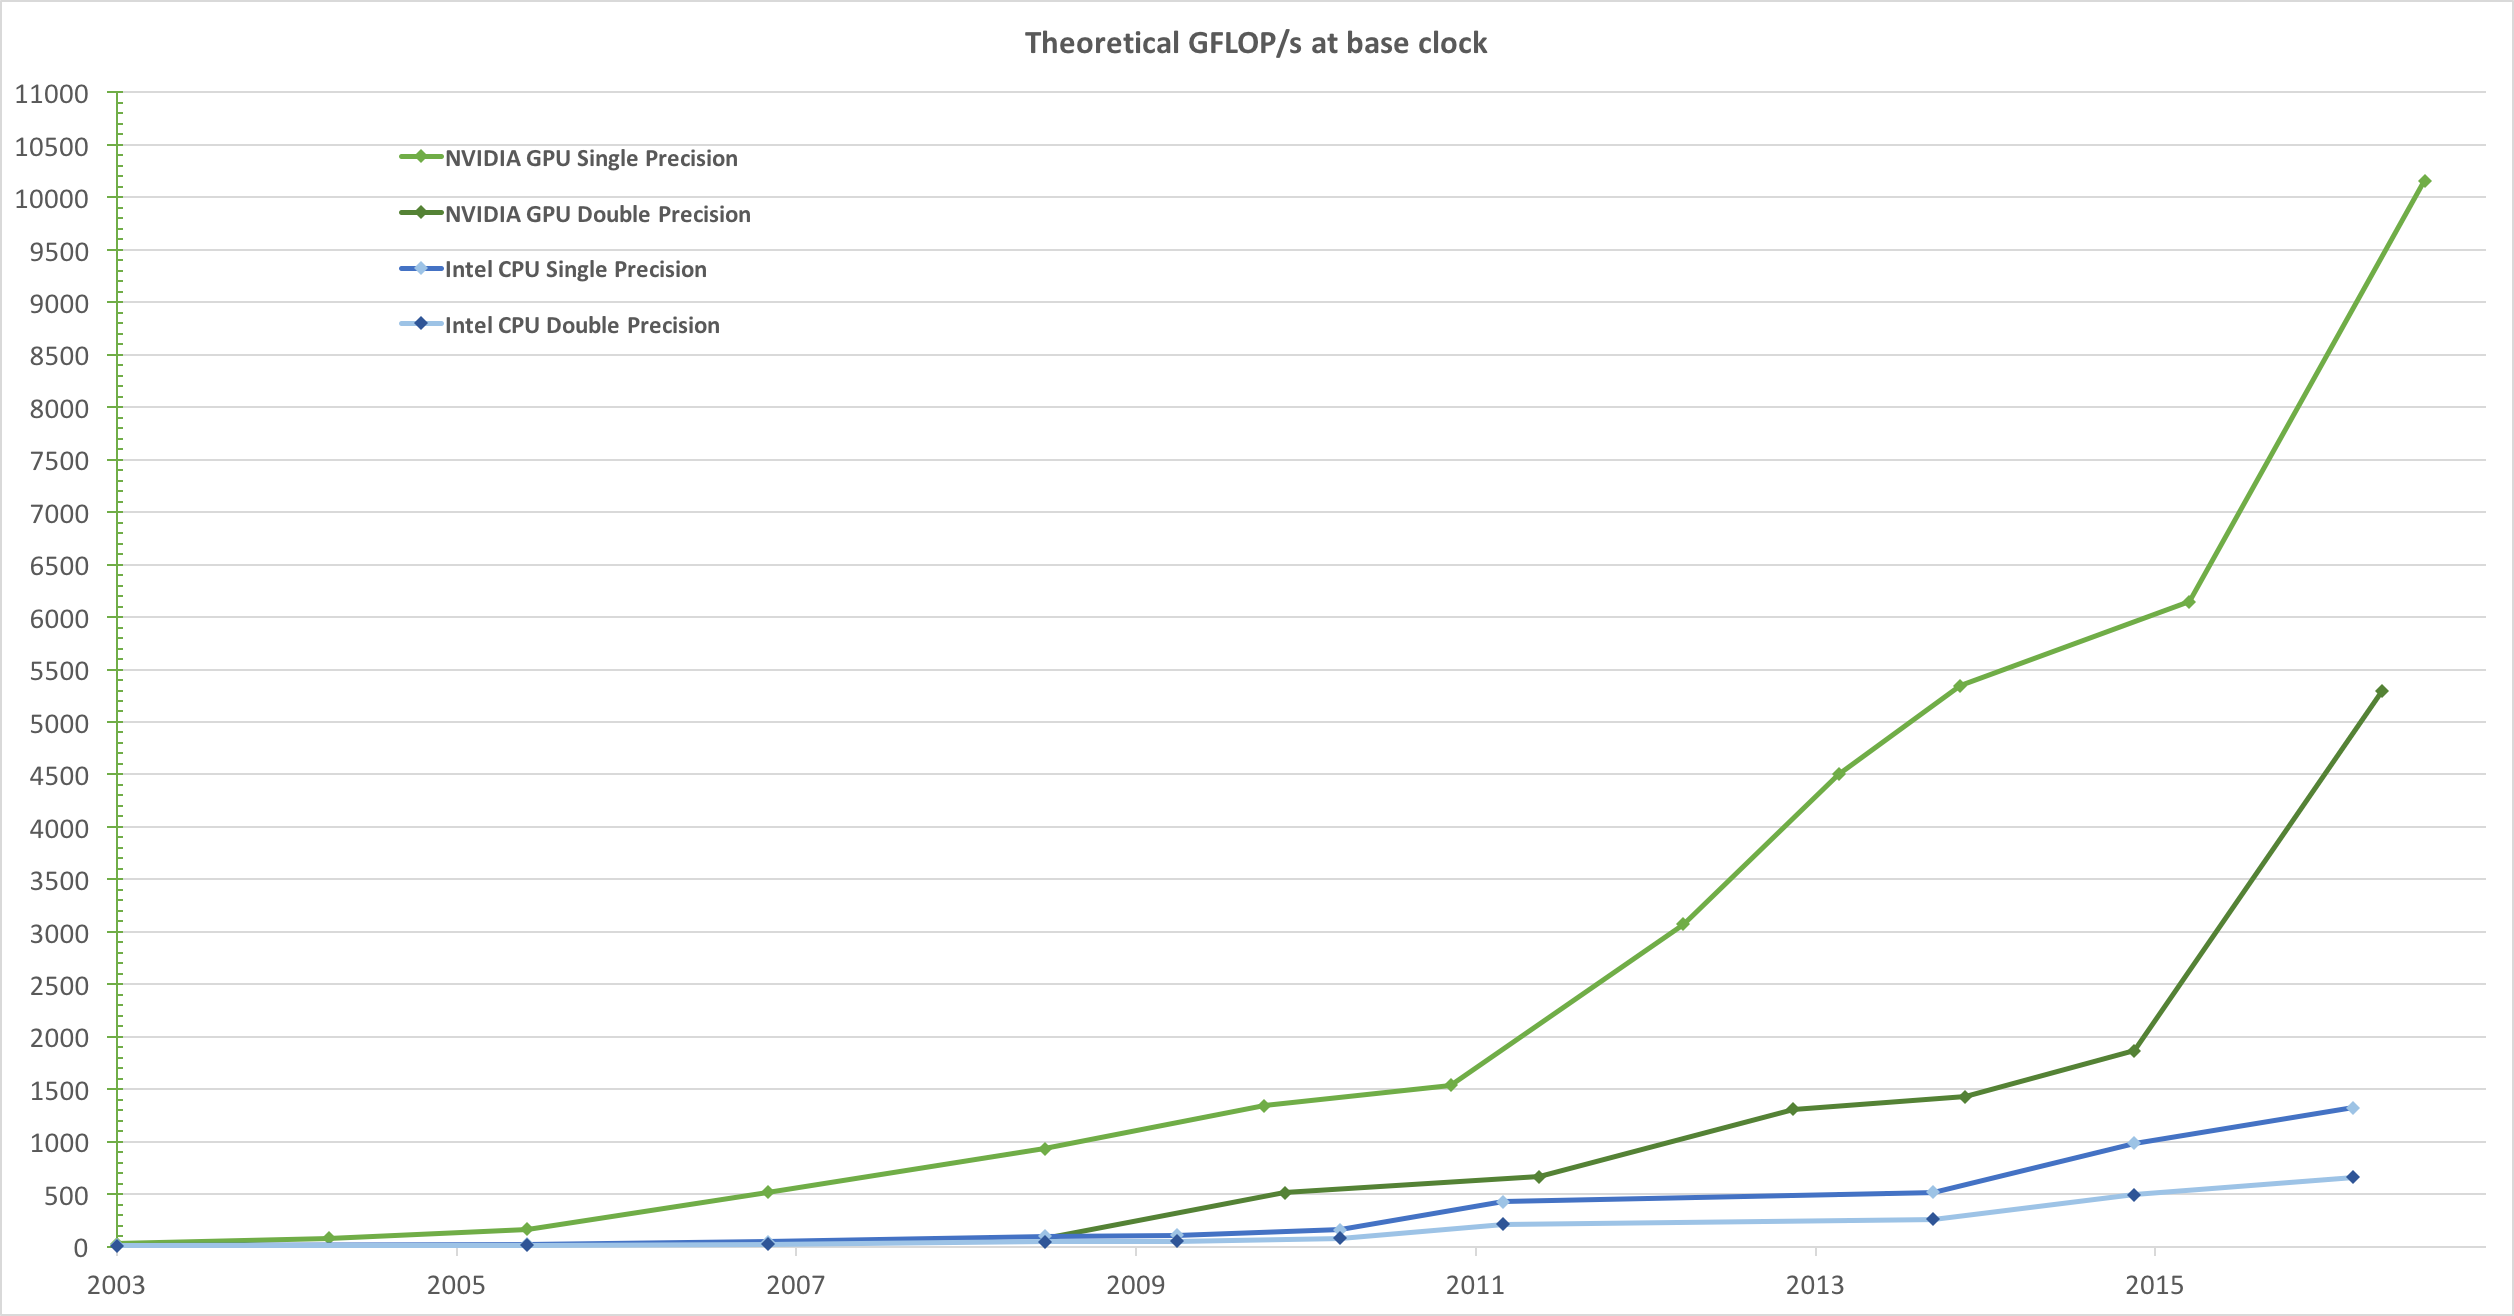
\includegraphics[width=0.90\textwidth]{./img/theoretical-gflops.png}
	    \caption{\small{Theoretical GFLOP/s: GPUs vs. CPUs.\newline\footnote{https://docs.nvidia.com/cuda/archive/9.1/pdf/CUDA\_C\_Programming\_Guide.pdf}}}
     \end{figure}
     \end{columns}

\end{frame}	

\begin{frame}
	\frametitle{CPU processor trend (last 50 years)}
  \begin{columns}
  \column{0.9\textwidth}
    \begin{figure}[H]
       \centering
            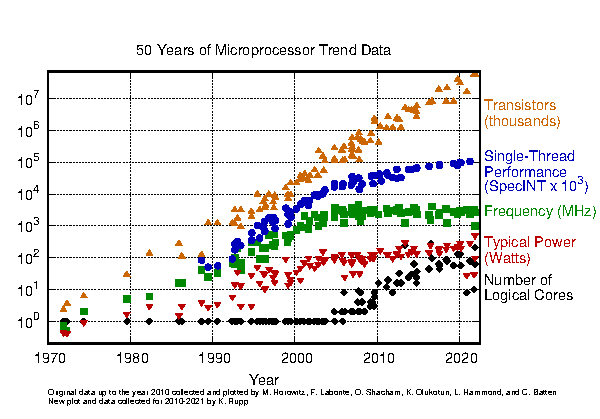
\includegraphics[width=0.80\textwidth]{./img/50-years-processor-trend.pdf}
     \end{figure}
     \end{columns} 
      \begin{itemize} 
         \item After the year $2000$, \texttt{freq.}/\texttt{power} 
		 for a single CPU core reaches a max. (\textcolor{red}{\textbf{Heat dissipation!}}).
      \end{itemize}
\end{frame} 

\begin{frame}
	\frametitle{Energy efficiency per job: GPU vs. CPU}
  \begin{columns}
  \column{0.9\textwidth}
    \begin{figure}[H]
       \centering
            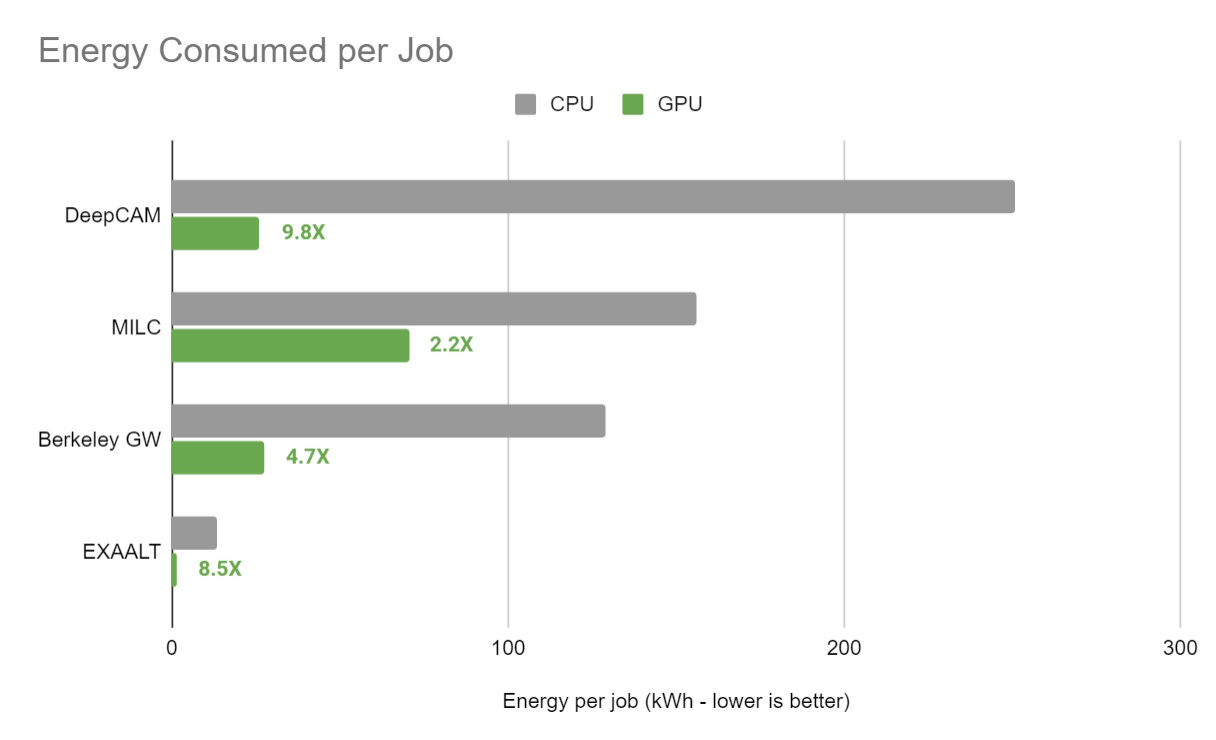
\includegraphics[width=0.80\textwidth]{./img/NERSC-energy-efficiency-findings.jpg} 
	    \caption{\small{Energy efficiency per job (NERSC).\newline\footnote{https://blogs.nvidia.com/blog/gpu-energy-efficiency-nersc/ (05/21/2023)}}}
     \end{figure}
     \end{columns}
\end{frame}
    % Motivation
\section{Hardware}

% NOTE: The easiest way to find the hardware specifics of a device
%       is to run the deviceQuery executable (cuda-samples)
%   git clone https://github.com/NVIDIA/cuda-samples.git
%   cd cuda-samples
%   make -j 6
%   cd bin/x86_64/linux/release
%   ./deviceQuery


% NOTE 2:
%  Ampere A100:
%    https://images.nvidia.com/aem-dam/en-zz/Solutions/data-center/nvidia-ampere-architecture-whitepaper.pdf
%    https://developer.nvidia.com/blog/nvidia-ampere-architecture-in-depth/

%  Hopper H100:
%    https://developer.nvidia.com/blog/nvidia-hopper-architecture-in-depth/

%  Blackwell B100:
%    https://resources.nvidia.com/en-us-blackwell-architecture

%  Will be succeeded by the Rubin generation (R100/R200)
%    https://blogs.nvidia.com/blog/computex-2024-jensen-huang/

\subsection{Streaming multiprocessor (SM)}
\begin{frame}
\frametitle{Streaming Multiprocessor (SM)}
\begin{itemize}
\item GPU device connected to the CPU by a PCIe bus. 
\item each GPU device contains an array (\textcolor{red}{$\mathbf{x}$}) of Streaming Multiprocessors \textbf{(SM)}.
\item each SM has:
\begin{itemize}
   \item a Single-Instruction Multiple-Thread (\texttt{SIMT}) Architecture.
   \item contains \textcolor{red}{$\mathbf{y}$} regular cores and [\textcolor{red}{$\mathbf{z}$} tensor cores].
\end{itemize} 
\item scalable: newer generations: increase of \textcolor{red}{$\mathbf{x}$}, \textcolor{red}{$\mathbf{y}$} 
	and [\textcolor{red}{$\mathbf{z}$}], e.g.:
   \begin{itemize}
	   \item \texttt{NVIDIA A100-PCIE-40GB} (\textit{notch293})
         \begin{itemize}
            \item global memory: $40$ GB.			 
            \item $108$ SMs, $64$ Cores/SM, $4$ Tensor Cores/SM.
            \item GPU Max. Clock Rate: $1.41$ GHz.
         \end{itemize}		   
 \item \texttt{NVIDIA H100 SXM5 NVL} (\textit{grn008})	
         \begin{itemize}
            \item global memory: $93$ GB.			 
            \item $132$ SMs, $128$ Cores/SM, $4$ Tensor Cores/SM.
	    \item GPU Max. Clock Rate: $1.78$ GHz. 
         \end{itemize}
   \end{itemize}		   
\end{itemize}
\end{frame} 

% NOTE: 
\begin{frame}
	\frametitle{\texttt{NVIDIA GH100 SM}} 
    \begin{columns}
	\column{0.50\textwidth}
    \begin{figure}[H]
       \centering
	    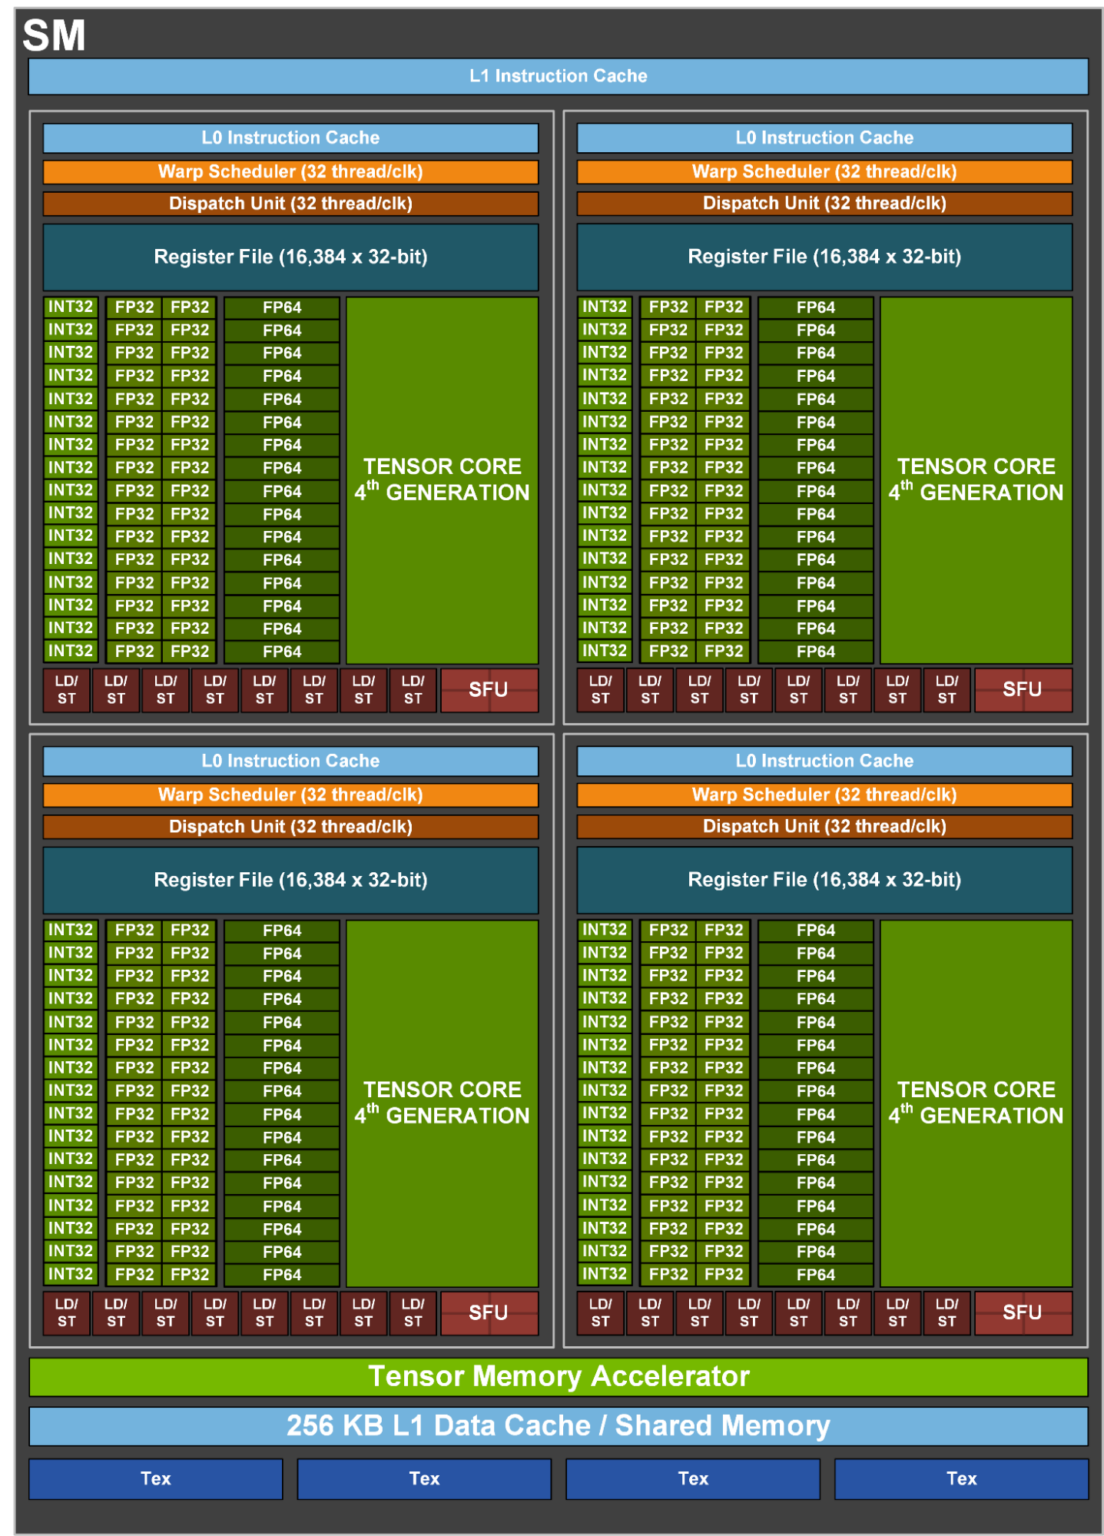
\includegraphics[width=0.80\textwidth]{./img/H100-Streaming-Multiprocessor-SM-1104x1536.png}
	    \caption{\small{GH100 SM}}
     \end{figure}
     \end{columns}
\end{frame}

\begin{frame}
        \frametitle{\texttt{NVIDIA GH100 Full Device}}
    \begin{columns}
        \column{0.90\textwidth}
    \begin{figure}[H]
       \centering
	    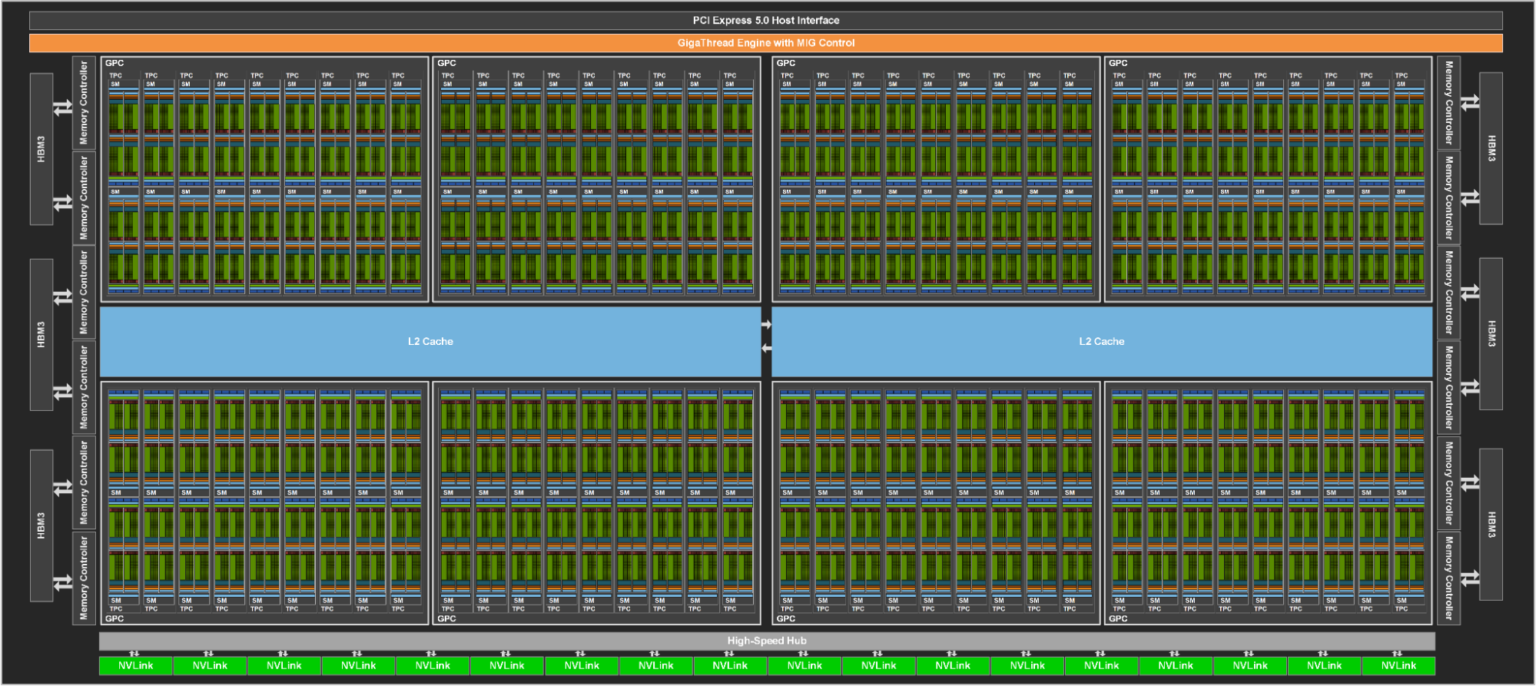
\includegraphics[width=0.90\textwidth]{./img/Full-H100-GPU-with-144-SMs-1536x686.png}
	    \caption{\small{NVIDIA GH100 Full Device ($144$ SMs).}}
     \end{figure}
     \end{columns}
\end{frame}

\subsection{Warps}
\begin{frame}
\frametitle{GPU Threads - Warps}	
\begin{itemize}
  \item Each SM:	
  \begin{itemize}
     \item generates, schedules, executes threads in batches of $32$ threads.
     \item \textbf{WARP}: a batch of $32$ threads
  \end{itemize}
  \item each thread in a WARP executes the same instructions but runs its own "path".
  \item if threads within a WARP diverge, the threads become inactive/disabled.
\end{itemize}	   
\end{frame} 
      % GPU Architecture
\section{Software}
\subsection{GPGPU \& CUDA}
\begin{frame}
  \frametitle{GPGPU \& CUDA}
     \begin{itemize}
        \item GPU (Graphic Processing Unit):\newline 
	      orginally developed for graphical applications.
        \item GP-GPU: General-Purpose GPU, i.e.\newline 
	      the use of GPUs beyond graphical applications.\newline
	      \textbf{\textcolor{red}{CAVEAT}}: problem to be reformulated in terms of the graphics API.
      \item \textbf{\textcolor{green}{2006}}: NVIDIA introduces the \textbf{\textcolor{blue}{CUDA}}\footnote{The \href{https://developer.nvidia.com/cuda-downloads}{CUDA Toolkit} consists of $2$ parts: 
      \begin{itemize} 
	      \item CUDA Driver 
	      \item CUDA Toolkit (\texttt{nvcc,nvprof}, \ldots, libraries, header files).
      \end{itemize} } framework\newline 
		(\textbf{\textcolor{blue}{C}}ompute \textbf{\textcolor{blue}{U}}nified 
		     \textbf{\textcolor{blue}{D}}evice \textbf{\textcolor{blue}{A}}rchitecture) 
              \begin{itemize}
	         \item CUDA API: extension of the \texttt{C} language.
                 \item handles the GPU thread level parallelism
                 \item deals with moving data between CPU and GPU.
		 \item also support for \CC\,, \texttt{Fortran}.			 
              \end{itemize}			 
     \end{itemize}		     
\end{frame}	

% Matrix Multiplication
%   consists of concepts of threads.
\subsection{Introducing CUDA concepts: case of matrix mul.}
% Step 1: consists of the concept of a kernel (__device__,__global__,..), threads
%         and how to transfer the data from the GPU and CPU. 
%         cudaMalloc, cudaMallocManaged (unified memory)
% Step 2: introduces the concept of the blocks and grids
%         
% Step 3: Introduces the concept of shared memory (+__syncthreads())

\subsection{Warps}
\begin{frame}
\frametitle{GPU Threads - Warps}
\begin{itemize}
  \item Each SMP:
  \begin{itemize}
     \item generates, schedules, executes threads in batches of $32$ threads.
     \item \textbf{WARP}: a batch of $32$ threads
  \end{itemize}
  \item each thread in a WARP executes the same instructions but runs its own "path".
  \item if threads within a WARP diverge, the threads become inactive/disabled.
\end{itemize}
\end{frame}


% Compilation of the CUDA code
%   introducing -compute, -arch
\subsection{Compiling CUDA code \& useful env. variables} 

%   nvprof, nvsight, cuda-gdb
\subsection{Debugging \& profiling your CUDA code}

% CUDA Libraries: CUBLAS, CUFFT, CUDNN, MAGMA, CURAND, NCCL
\subsection{Important CUDA Libraries}

% Alternatives:
%  - Within CUDA: CudaFortran, OpenAcc (pragmas)
%  - Alternatives to CUDA: OpenCL, HIP
%  - Kokkos
\subsection{Alternatives for CUDA}

\subsection{Links}
\begin{frame}
   \frametitle{Links}
      \begin{itemize}
	      \item \href{https://docs.nvidia.com/cuda/index.html}{CUDA Toolkit Documentation}
              \item \href{https://docs.nvidia.com/cuda/cuda-c-programming-guide/index.html}{CUDA \CC\, Programming Guide}
	      \item \href{https://docs.nvidia.com/cuda/cuda-c-best-practices-guide/index.html}{CUDA \CC\, Best Practices Guide}	      
      \end{itemize}		      
\end{frame}	

      % Software
% Matrix Multiplication
%   consists of concepts of threads.
\subsection{Case study: matrix multiplication}
% Step 1: consists of the concept of a kernel (__device__,__global__,..), threads
%         and how to transfer the data from the GPU and CPU. 
%         cudaMalloc, cudaMallocManaged (unified memory)
\begin{frame}
	\frametitle{Matrix Mul.: kernel (v.\,$1$)}
	\textbf{\textcolor{blue}{Case study}}: $P=MxN$ where $P,M,N$ $\in \mathbb{R}^{nxn}$
	\lstinputlisting[style=MyCudaStyle, basicstyle=\tiny, 
	                 caption={\texttt{Kernel (v.\,$1$)}}]{./latexinc/matmul/1/mul.cu}
\end{frame}

\begin{frame}
	\frametitle{Invoking kernel (v.\,$1$)}
	\begin{itemize}
		\item Invoking $1$ Block of Threads
        \lstinputlisting[style=MyCudaStyle, basicstyle=\tiny, 
	                 caption={\texttt{Invoking kernel (v.\,$1$)}}]{./latexinc/matmul/1/main-sel.cu}
        \end{itemize}			 
\end{frame}

% Step 2: Kernel using more than 1 block of threads
%  
\begin{frame}
	\frametitle{Mat. Mul (v.$2$): Grid of $2$D Blocks}
      \begin{itemize}
	 \item \lstinline[style=MyCudaStyle]{int tx = blockIdx.x*blockDim.x + threadIdx.x;} 		      
	 \item \lstinline[style=MyCudaStyle]{int ty = blockIdx.y*blockDim.y + threadIdx.y;} 		      
      \end{itemize}		      
      \begin{columns}
        \column{0.50\textwidth}
           \begin{figure}[H]
              \centering
              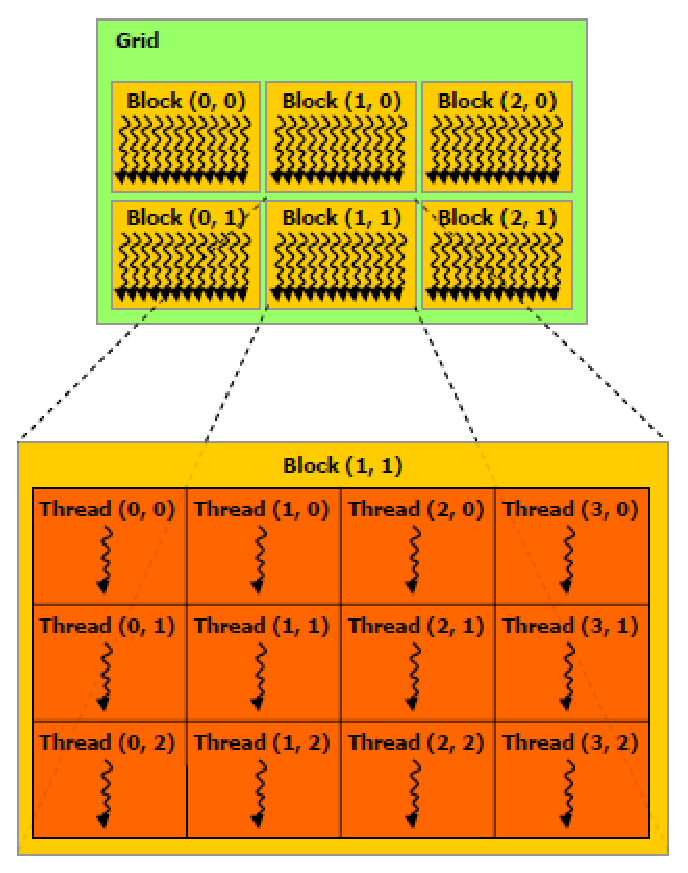
\includegraphics[width=0.75\textwidth]{./img/BlockGrid.eps}
              \caption{\small{$2$D-Grid of $2$D-Blocks of Threads}}
           \end{figure}
     \end{columns}
\end{frame}

\begin{frame}
	\frametitle{Matrix Mul.: visualization (v.\,$2$)}
      \begin{columns}
        \column{0.85\textwidth}
           \begin{figure}[H]
              \centering
              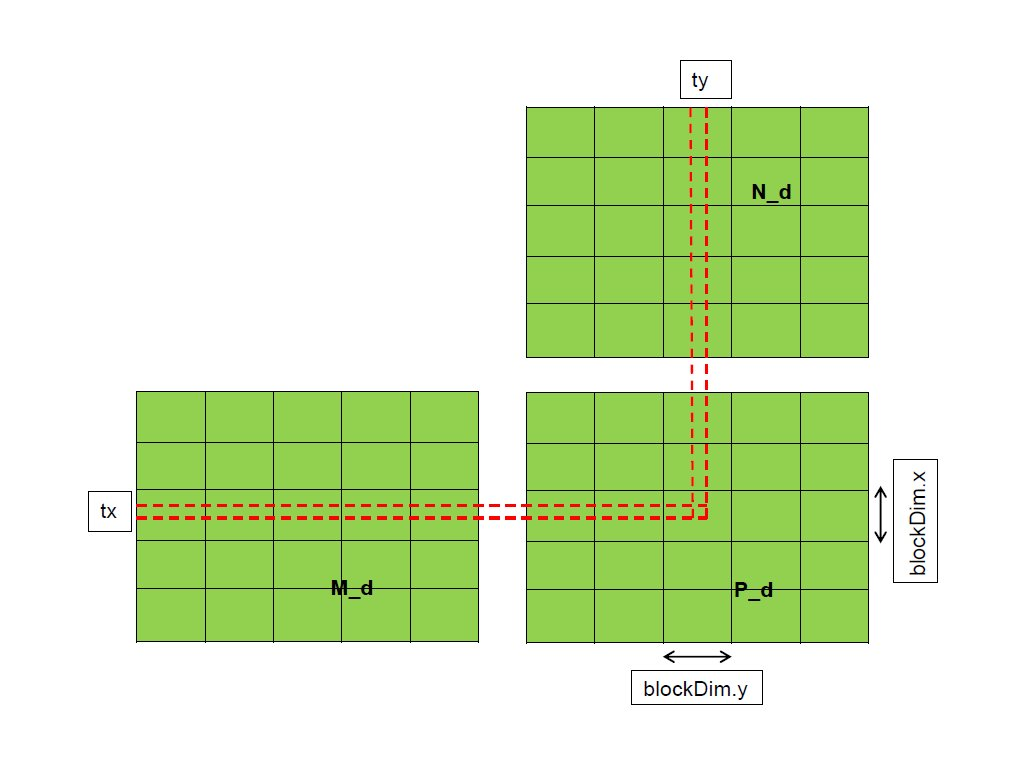
\includegraphics[width=0.85\textwidth]{./img/mulB.jpg}
		   \caption{\small{Matrix Mul. ($2$D Grid)}}
           \end{figure}
     \end{columns}
\end{frame}


\begin{frame}
        \frametitle{Matrix Mul.: kernel (v.\,$2$)}
        \lstinputlisting[style=MyCudaStyle, basicstyle=\tiny,
                         caption={\texttt{Kernel (v.\,$2$)}}]{./latexinc/matmul/2/mul.cu}
\end{frame}

\begin{frame}
        \frametitle{Invoking kernel (v.\,$2$)}
        \begin{itemize}
                \item Invoking a grid of blocks of threads
        \lstinputlisting[style=MyCudaStyle, basicstyle=\tiny,
                         caption={\texttt{Invoking kernel (v.\,$2$)}}]{./latexinc/matmul/2/main-sel.cu}
        \end{itemize}
\end{frame}


% Step 3: Introduces the concept of shared memory (+__syncthreads()) 
\begin{frame}
\frametitle{Types of GPU memory}
\begin{itemize}
   \item \textbf{\textcolor{blue}{global memory}}: (largest, slowest and often the bottleneck).
   \item \textbf{\textcolor{blue}{shared memory}}: allocated per thread block \& low latency
   \item \textbf{\textcolor{blue}{constant memory}}: cached, read-only
   \item \textbf{\textcolor{blue}{registers}}: fast, on-chip memory (exclusive to each thread).
\end{itemize}
\end{frame}


\begin{frame}
   \frametitle{Matrix Mul.: use of shared memory (v.\,$3$)}
      \begin{columns}
        \column{0.85\textwidth}
           \begin{figure}[H]
              \centering
              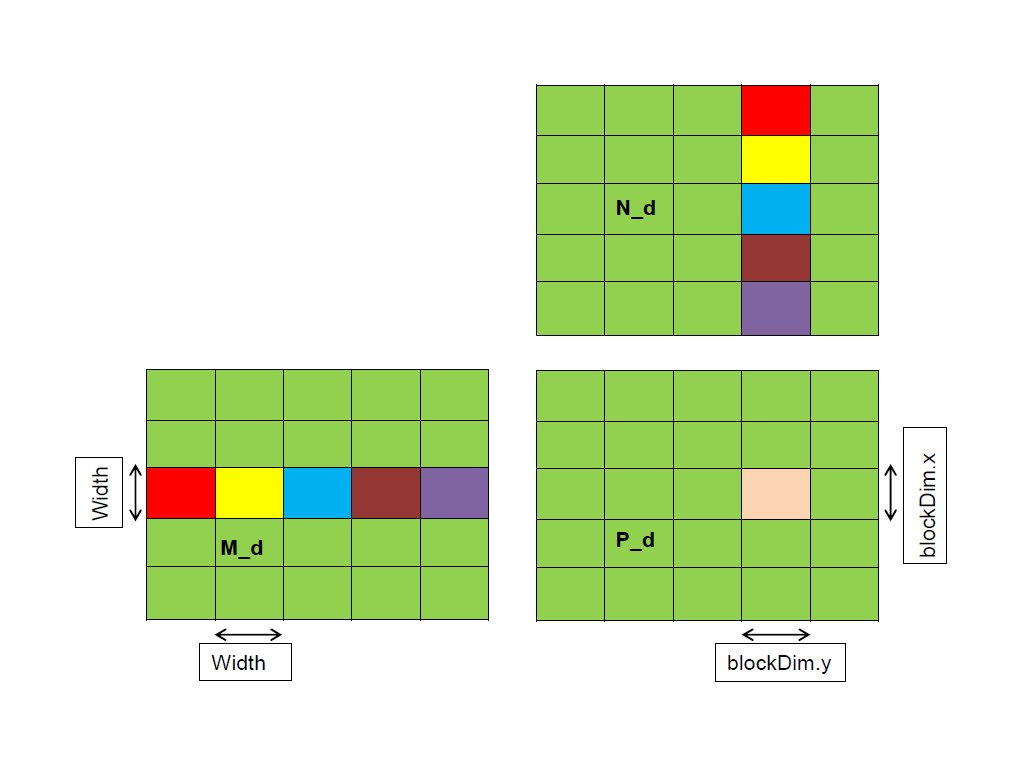
\includegraphics[width=0.85\textwidth]{./img/mulC.jpg}
                   \caption{\small{Matrix Mul.: use of shared memory}}
           \end{figure}
     \end{columns}
\end{frame}

	
\begin{frame}
        \frametitle{Matrix Mul.: kernel (v.\,$3$) - use of shared memory}
        \lstinputlisting[style=MyCudaStyle, basicstyle=\tiny,
                         caption={\texttt{Kernel (v.\,$3$)}}]{./latexinc/matmul/3/mul.cu}
\end{frame}


% Compilation of the CUDA code
%   introducing -compute, -arch
\subsection{Building CUDA applications \& useful env. variables} 
\begin{frame}
   \frametitle{Building/Compiling CUDA applications}
      General scheme:
      \begin{itemize}
         \item Source code for CUDA applications:
            \begin{itemize}		 
	       \item \texttt{C}/\CC\ host code with extensions to deal with the device(s). 
	       \item Other programming languages are allowed e.g. \texttt{Fortran} 
            \end{itemize}	
         \item Primo: \textbf{\textcolor{green}{separate}} device functions from host code.
         \item \textbf{\textcolor{green}{Device code}}: preprocessing, compilation 
	       with the NVIDIA compiler (\texttt{nvcc}).		 
         \item \textbf{\textcolor{green}{Host code}}: preprocessed, compiled with a host (\texttt{C}/\CC) 
	       compiler e.\,g.\,(\texttt{gcc, g++, icc, icpc, \ldots})
	 \item Compiled device functions are \textbf{\textcolor{green}{embedded}} as \texttt{fatbinary} 
	       images in the host object file.
         \item \textbf{\textcolor{green}{Linking stage}}: adding CUDA runtime libraries 
	       to the host object file to create an executable.
      \end{itemize}		      
\end{frame}


\begin{frame}
   \frametitle{Further concepts}
      \begin{itemize}
	 \item \texttt{.cu} : Suffix for CUDA source file (host code (\texttt{C},\CC) \& device code).
	 \item \texttt{.cuf}: Suffix for CUDA source file (host code (\texttt{Fortan}) \& device code).
	 \item \texttt{.ptx}: Suffix for \textbf{P}arallel \textbf{T}hread E\textbf{x}ecution (\texttt{PTX}) files. 
		 An intermediate representation (similar to assembly for a 
		      \textbf{\textcolor{blue}{virtual GPU architecture}}\footnote{Virtual architectures 
		      bear the \quotes{\texttt{compute\_}} \textbf{\textcolor{green}{prefix}} e.\,g.\,\quotes{\texttt{compute\_70}}.}
	 \item \texttt{.cubin}: Suffix for the \textbf{CU}DA device \textbf{bin}ary 
		 file pertaining to a \textbf{\textcolor{blue}{real GPU architecture}}\footnote{Real (physical) architectures
		      bear the \quotes{\texttt{sm\_}} \textbf{\textcolor{green}{prefix}} e.\,g.\,\quotes{\texttt{sm\_70}}.\\
		      \hspace{4ex}\textcolor{orange}{Memento}: \quotes{\texttt{sm}} stands 
		      for the physical streaming multiprocessor.}
	 \item \texttt{fatbin}: Multiple \texttt{PTX} [\& \texttt{cubin}] files are merged into a \texttt{fatbin} file.
      \end{itemize}
\end{frame}	

\begin{frame}
   \frametitle{Compilation trajectory (cont.)}
      \begin{columns}
        \column{0.75\textwidth}
           \begin{figure}[H]
              \centering
              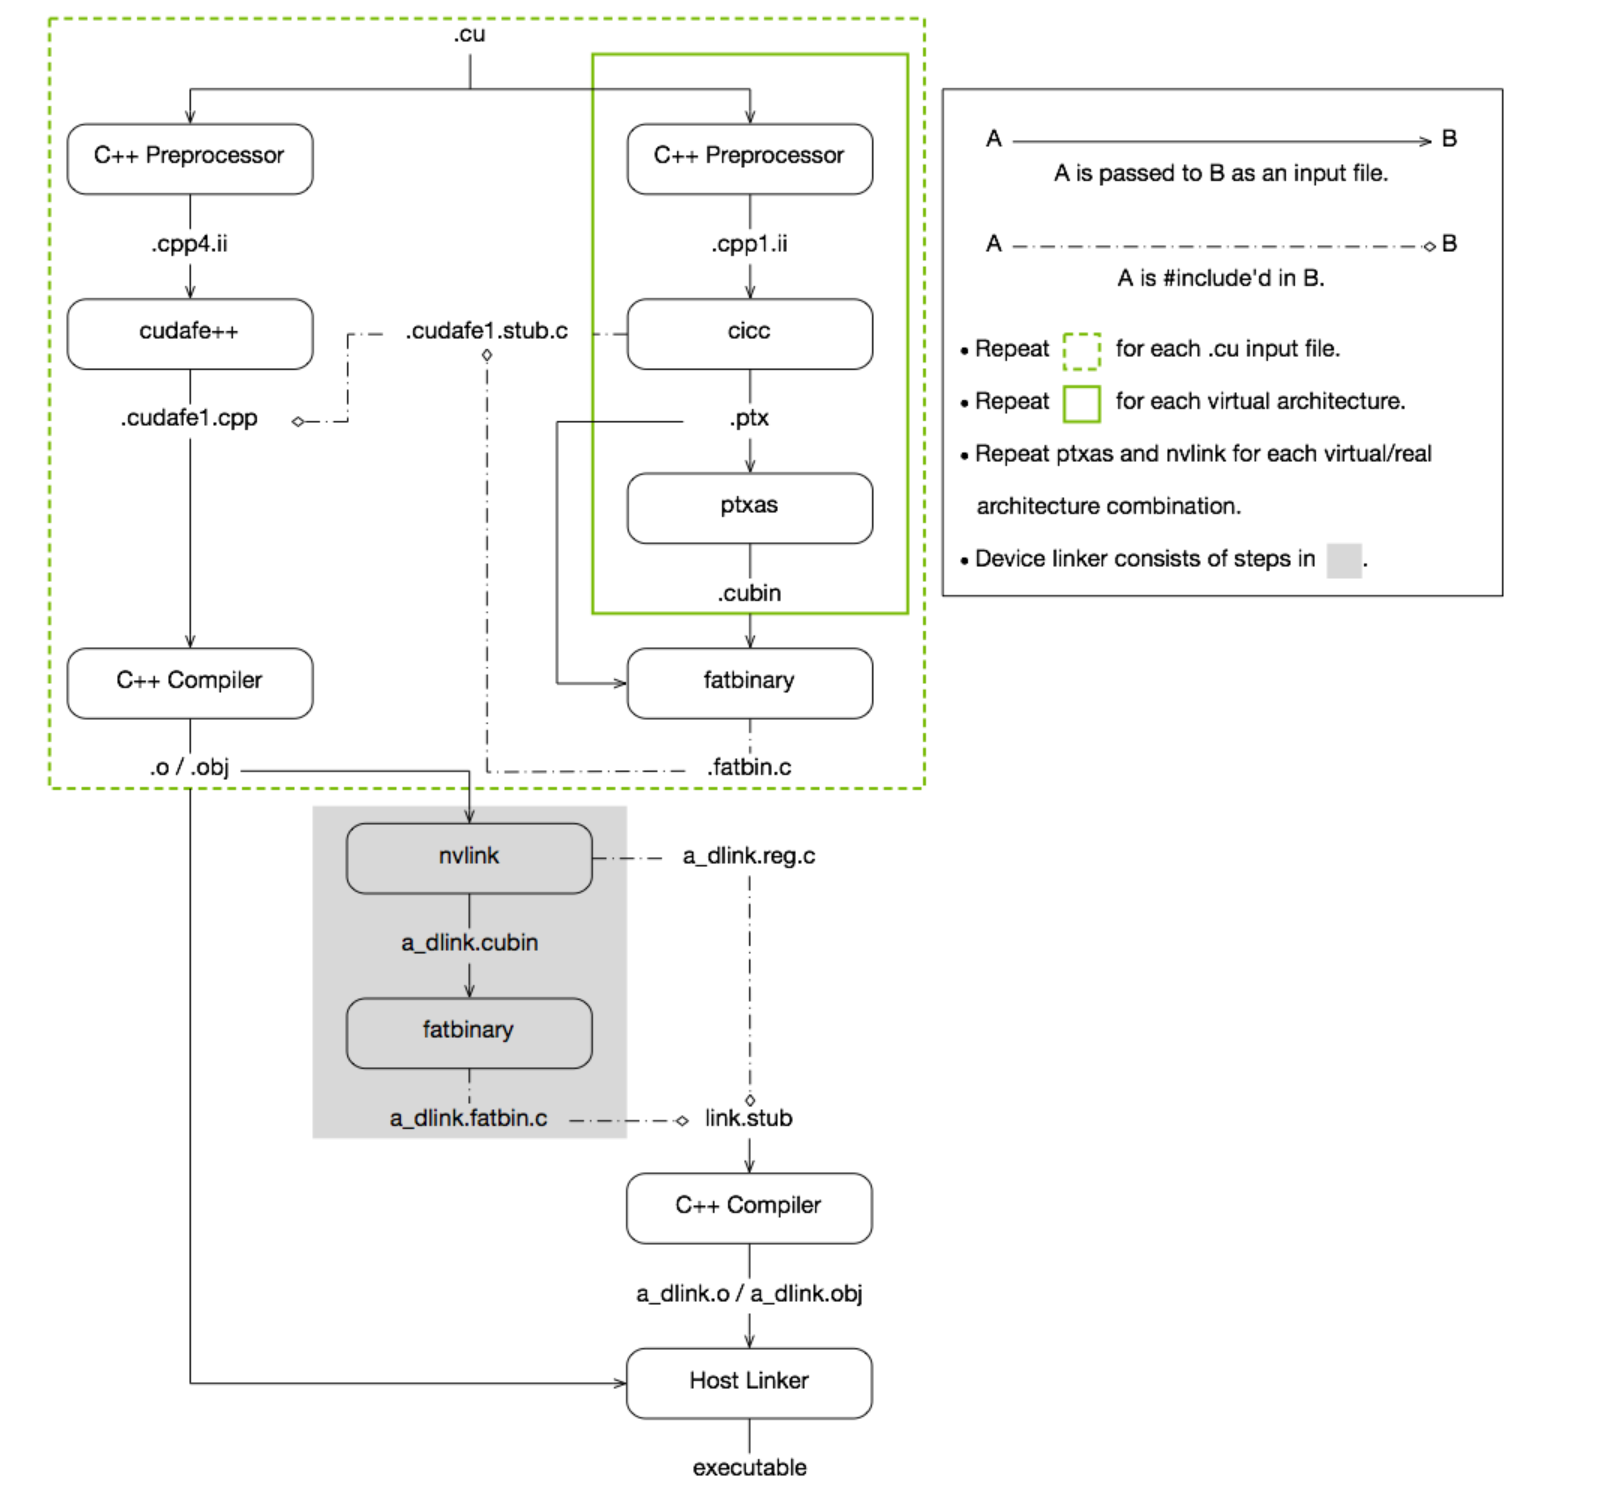
\includegraphics[width=0.65\textwidth]{./img/compileTrajectory.png}
	      \caption{\small{Compilation trajectory}}
           \end{figure}
        \end{columns}
\end{frame}     


% Still to be finished
\begin{frame}
   \frametitle{In praxi,}
      We will now address the following questions:
      \begin{itemize}  	
         \item What are the recent CUDA architectures
	 \item How to find the compute capability (CC) of a device
         \item How to build an executable for a particular device.
         \item How to build an executable for multiple architectures
      \end{itemize} 
\end{frame}


% https://docs.nvidia.com/cuda/cuda-compiler-driver-nvcc/index.html#gpu-compilation
\begin{frame}
  \frametitle{Recent CUDA Architectures/Generations}
      \begin{itemize}
	 \item NVIDA GPU: $xy$  $x$:generation (major) $y$: minor
         \item new generation: major improvement in functionality/chip 
	 \item \textbf{binary} compatibility is \textbf{NOT} garantueed among generations.		 
      \end{itemize}		      
      \begin{table}[H]
         \begin{center}
            \begin{tabular}{c|c|c|c}
		    \multirow{2}{*} \texttt{Architecture/}  & Year & \texttt{compute\_} & \texttt{sm\_} \\
				    \texttt{Generation}     &      & (\textit{virtual}) & (\textit{real}) \\
                   \hline
                      \texttt{Maxwell}      & 2014 & 50, 52, 53    & 50, 52, 53   \\
                      \texttt{Pascal}       & 2016 & 60, 61, 62    & 60, 61, 62 \\
                      \texttt{Volta}        & 2017 & 70, 72        & 70, 72 \\
                      \texttt{Turing}       & 2018 & 75            & 75 \\
                      \texttt{Ampere}       & 2020 & 80, 86, 87    & 80, 86, 87 \\
                      \texttt{Ada Lovelace} & 2022 & 89            & 89\\
                      \texttt{Hopper}       & 2022 & 90, 90a       & 90, 90a \\
                   \hline
            \end{tabular}
         \end{center}
         \caption{\small{Some of the recent CUDA architectures (10/08/2024)}}
      \end{table}
\end{frame}


% Finding the Compute Capability (CC) of GPU devices
\begin{frame}
	\frametitle{Retrieval of the Compute Compability (CC)}
      You can:	
      \begin{enumerate}
	      \item write some basic \texttt{C}/\CC\ code \footnote{Already available in \texttt{src/devicequery}.\\
		      \hspace{4ex}The name of the corresponding executable is \texttt{devinfo}}. 
   	    relying on the following \texttt{CUDA} APIs:\\
   	      \begin{itemize}    
  	         \item \lstinline[style=MyCudaStyle]|cudaGetDeviceCount(int *tot)|: \\
	  	       returns the number of devices on the localhost.
   	         \item \lstinline[style=MyCudaStyle]|cudaGetDeviceProperties(cudaDeviceProp *p, int idev)|: \\
		       returns information about the compute-device \lstinline[style=MyCudaStyle]|idev|.
              \end{itemize}
          \item use existing tools, e.\,g.\,\texttt{nvaccelinfo} 
		(part of \href{https://developer.nvidia.com/hpc-sdk}{NVIDIA HPC SDK}) 

          \item \textbf{\textcolor{orange}{Note:}}\\
               The \texttt{nvidia-smi} executable displays the architecture \\ 
		      but not the CC of the device(s): \\
               \texttt{nvidia-smi -q}		      
      \end{enumerate}
\end{frame}	


% Use of devinfo (based on my Own Code to be found in src/querydevice)
\begin{frame}
   \frametitle{Retrieval of CC through some simple CUDA APIs}
     \begin{columns}
        \column{0.70\textwidth}
    \begin{figure}[H]
       \centering
          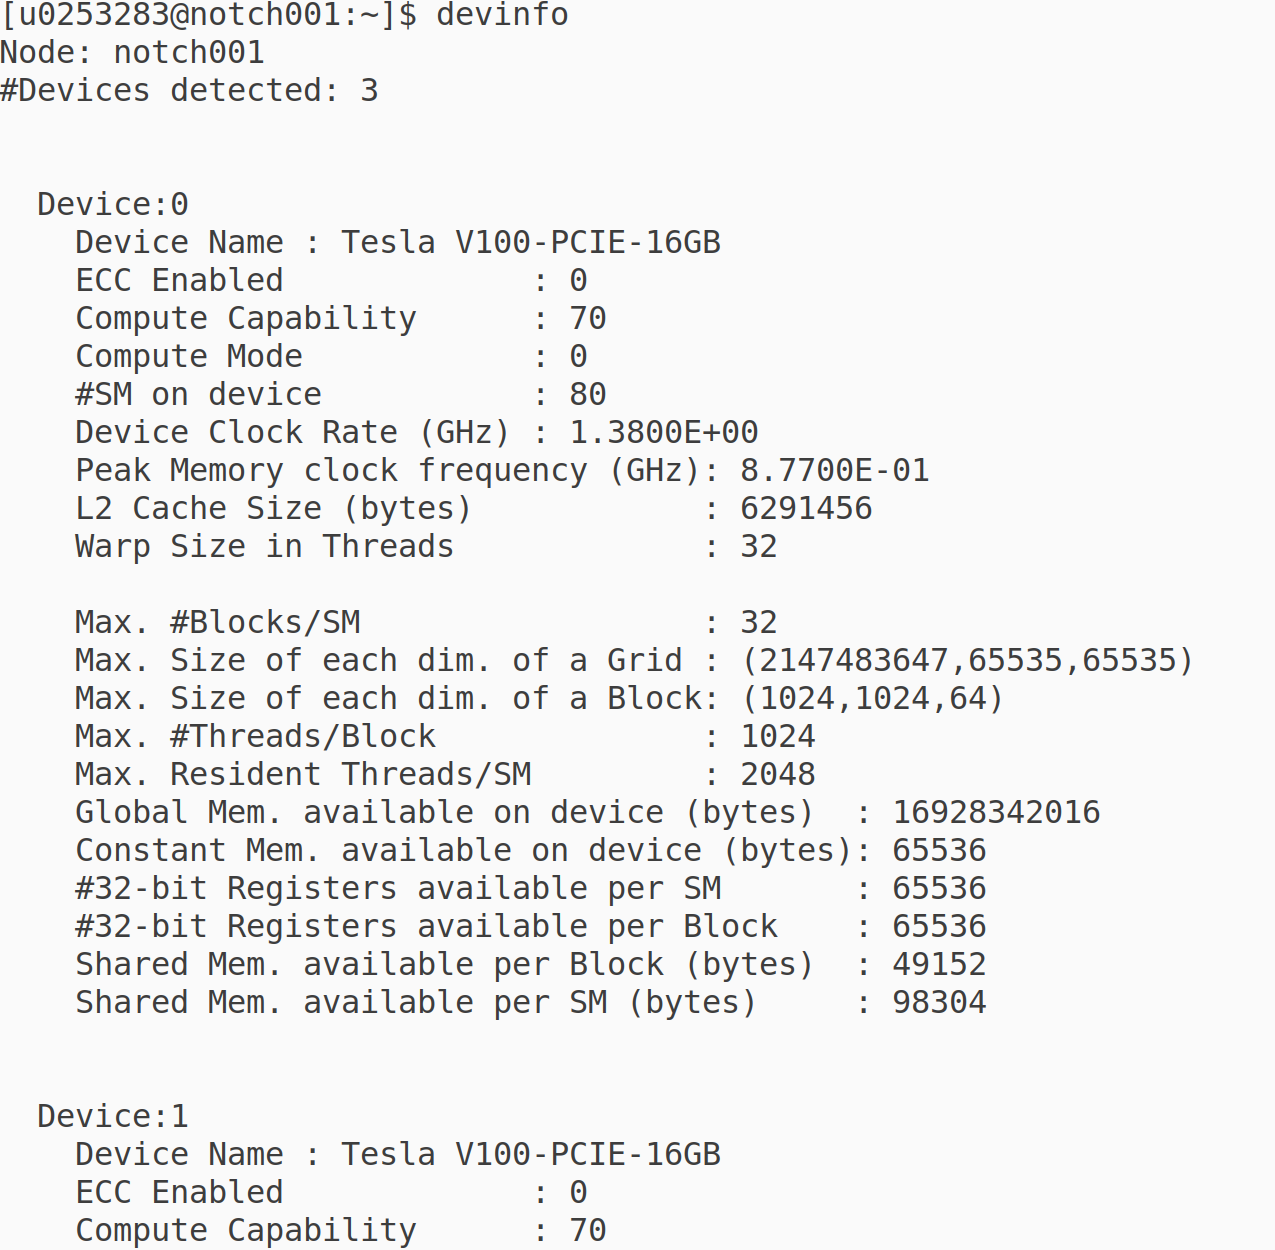
\includegraphics[width=0.70\textwidth]{./img/devinfo.png}
	    \caption{\small{\texttt{devinfo} based on a few CUDA APIs}}
     \end{figure}
     \end{columns}
\end{frame}


% Use of nvaccelinfo
\begin{frame}
	\frametitle{Retrieval of CC using \texttt{nvaccelinfo}}
     \begin{columns}
        \column{0.75\textwidth}
    \begin{figure}[H]
       \centering
          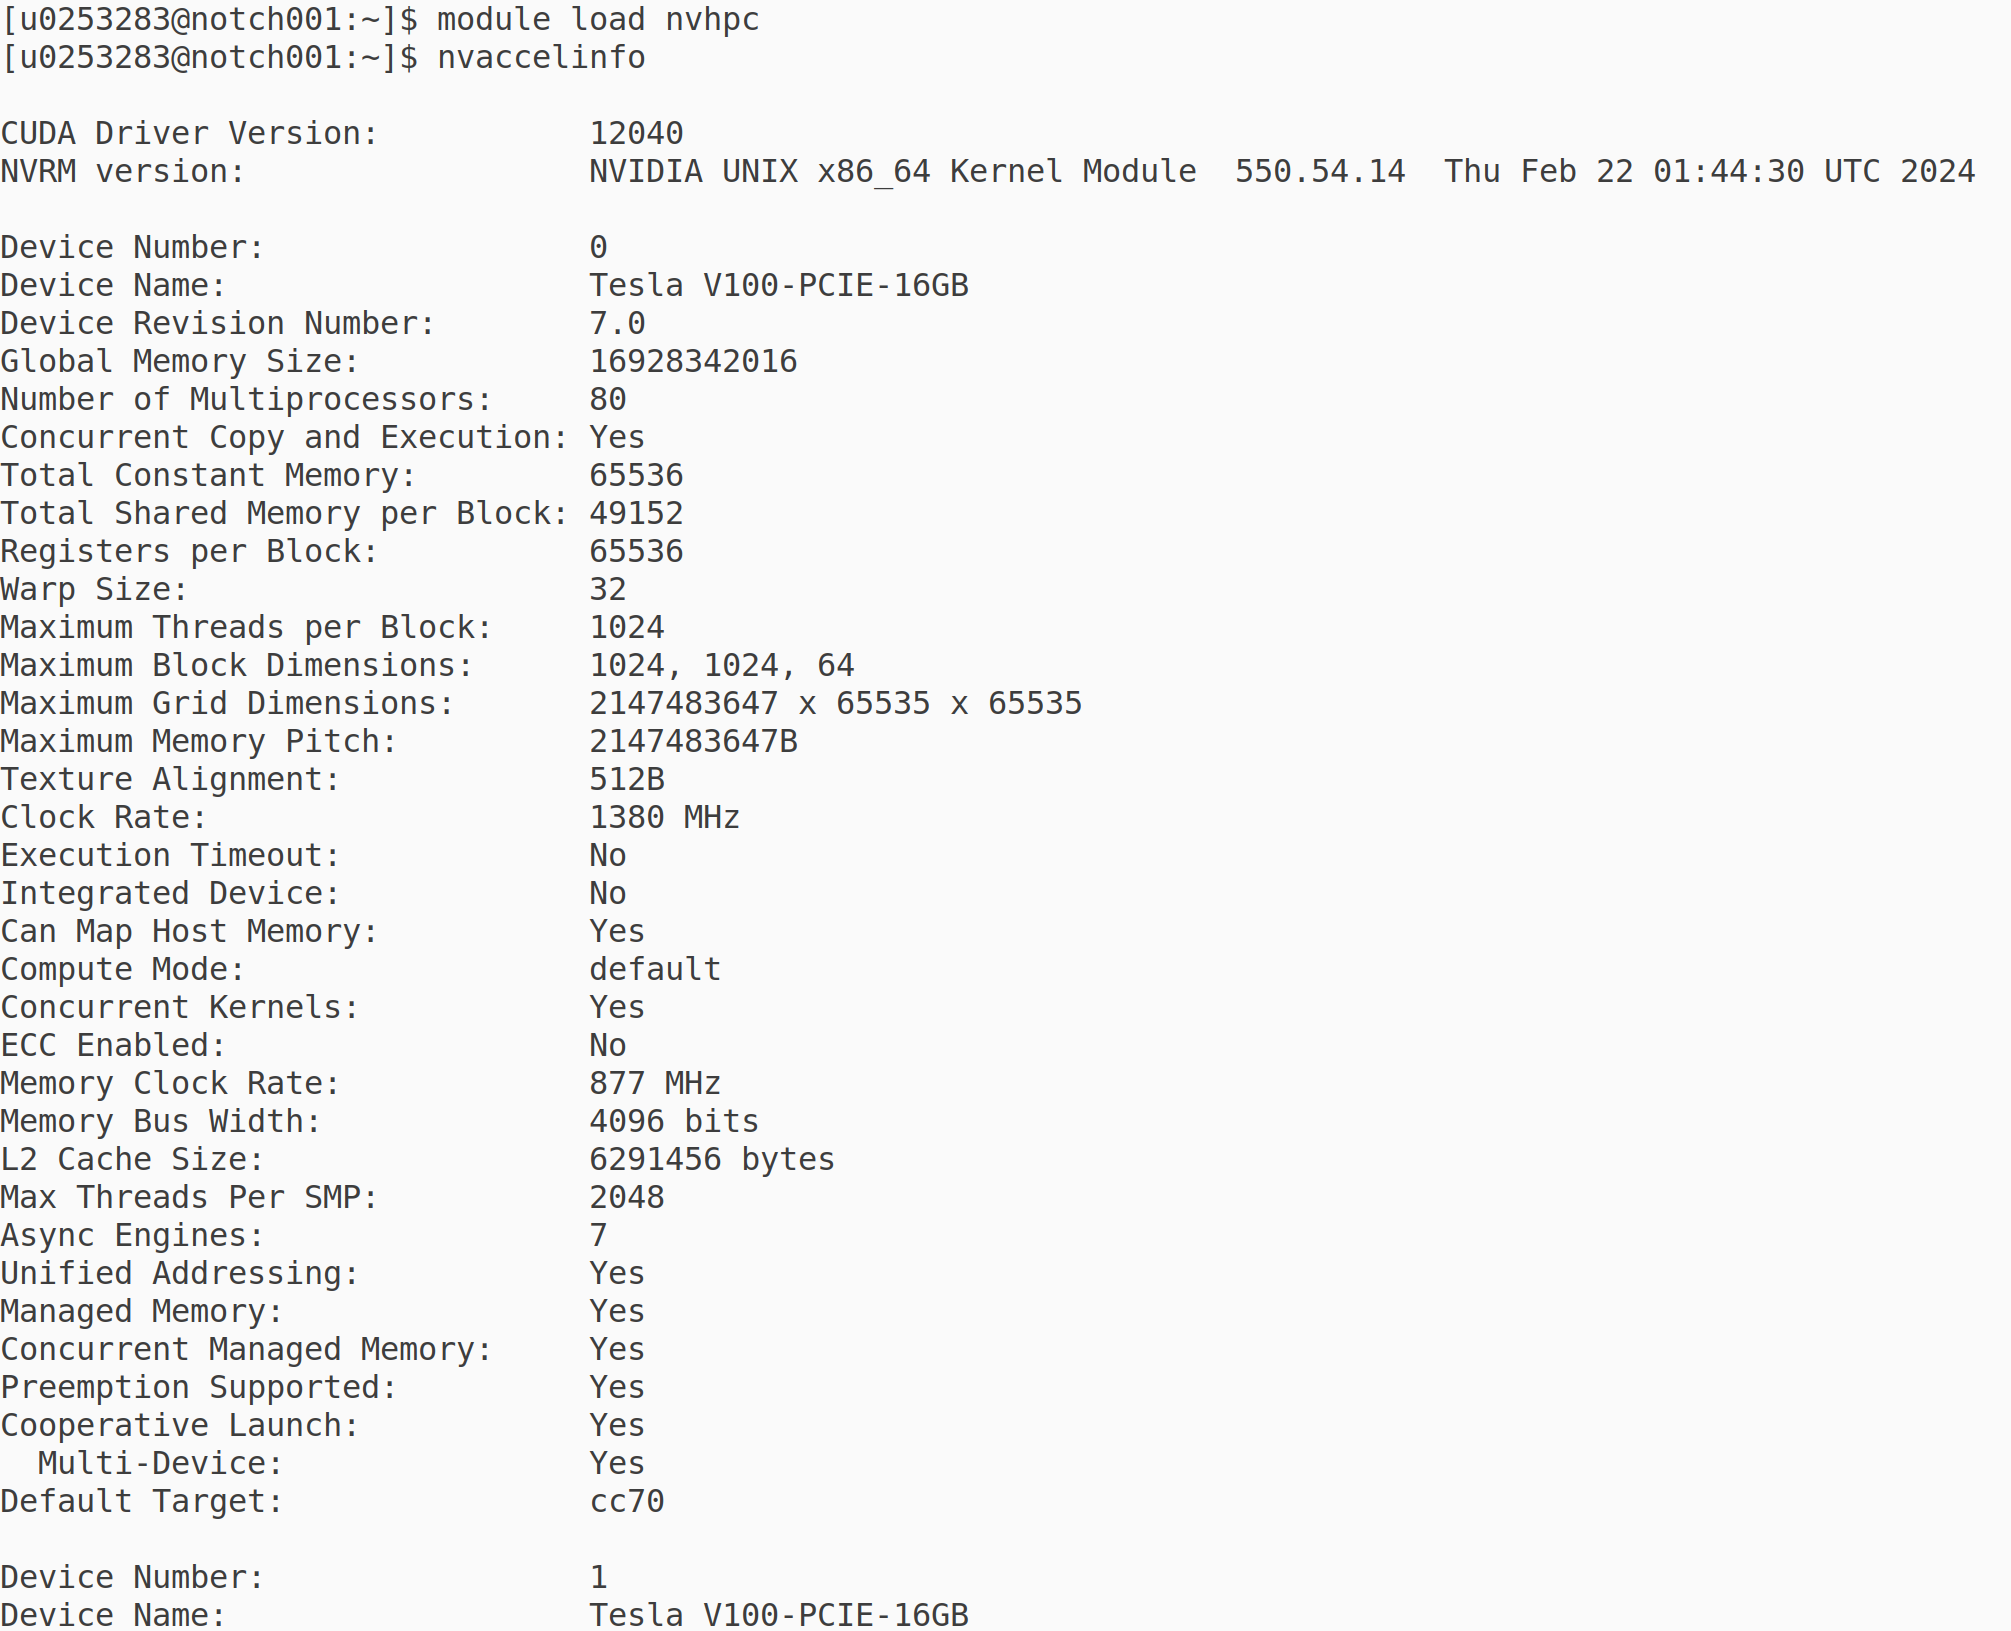
\includegraphics[width=0.75\textwidth]{./img/nvaccelinfo.png}
	    \caption{\small{Use of \texttt{nvaccelinfo} to retrieve \texttt{compute\_}}}
    \end{figure}
     \end{columns}
\end{frame}


% Use of nvidia-smi
\begin{frame}
        \frametitle{Use of \texttt{nvidia-smi}}
     \begin{columns}
        \column{0.85\textwidth}
    \begin{figure}[H]
       \centering
          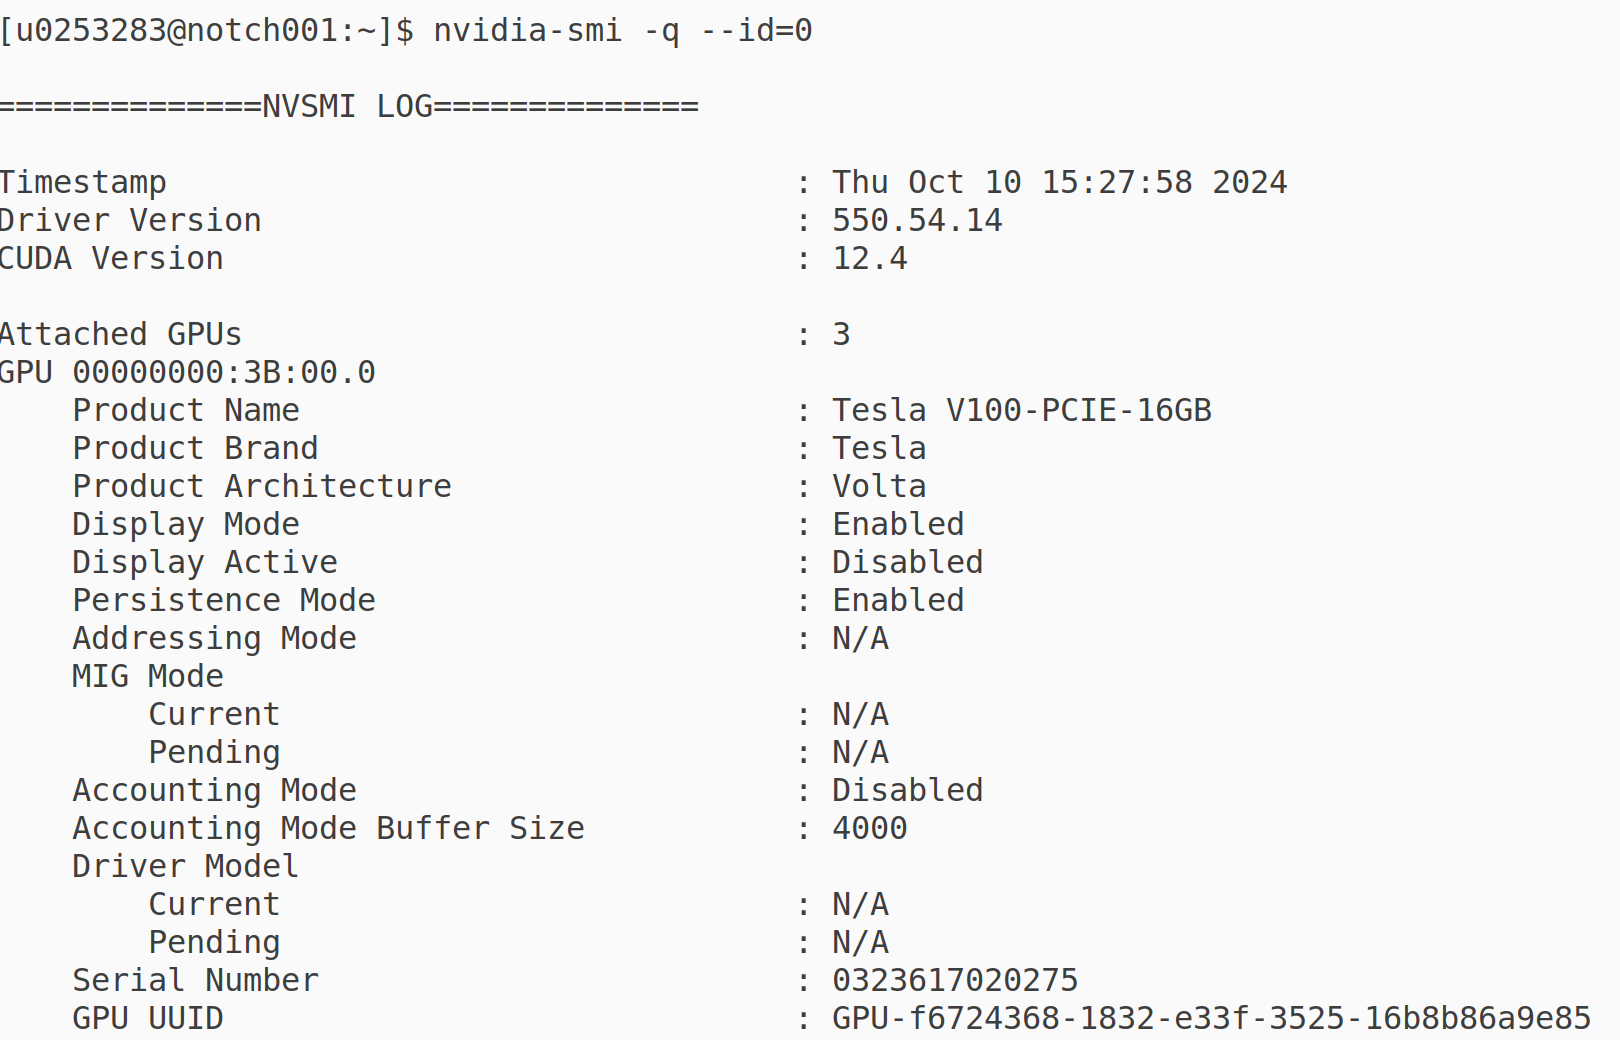
\includegraphics[width=0.85\textwidth]{./img/nvidia-smi.png}
          \caption{\small{\texttt{nvidia-smi}}}
    \end{figure}
     \end{columns}
\end{frame}



\begin{frame}
   \frametitle{Compiling your code for a particular device/devices}
      \begin{itemize}
         \item Compilation goes in $2$ steps:
            \begin{enumerate}
		    \item \texttt{PTX} representation: generic assembly instructions for a \\ 
			    \textit{virtual} (\textcolor{green}{\textbf{\texttt{compute\_}}} prefix) GPU architecture.\\
			    The resulting \texttt{.ptx} file is human readable (\textbf{text} file).
		    \item \texttt{Binary generation}: generation of an \textbf{object} file for the \\
			    \textit{real} (\textbf{\textcolor{green}{\texttt{sm\_}}} prefix) 
			    GPU architecture (based on the \texttt{PTX} file).		    
            \end{enumerate}
         \item \texttt{-arch}/\texttt{-code} flags
            \begin{itemize}
	       \item \texttt{--gpu-architecture|-arch <arch>}: specifies the name of \\ 
		       $1$ \textit{virtual} GPU architecture for which the code needs to be compiled.\\
			  e.\,g.\,\texttt{-arch=compute\_50}   
	       \item \texttt{--gpu-code|-code <arch>}: specifies the name(s) of the \textit{real}
			  GPU architecture(s) for which the binary needs to be compiled.\\
			    e.\,g.\,\texttt{-code=sm\_52}  
	    \end{itemize} 
      \end{itemize} 
\end{frame}

% See also:https://docs.nvidia.com/cuda/archive/11.6.1/cuda-compiler-driver-nvcc/index.html
\begin{frame}
    \frametitle{Compiling your code (cont.)}
      \begin{itemize}

         \item Therefore, choose $1$ virtual architecture and the accompanying real architectures\\
                         e.\,g.\, \texttt{-arch=compute\_50 -code=sm\_50,sm\_51,sm\_52}\\
               \begin{itemize}
   	          \item \texttt{PTX} file generated for the \texttt{compute\_50} (\textit{virtual}) arch.
	          \item \textbf{fatbinary} object created for the (\texttt{real}) arch. \texttt{sm\_50,sm\_51,sm\_52}        
               \end{itemize}

         \item \texttt{--generate-code|-gencode arch=<arch>,code=<code> \ldots} 
             \begin{itemize}		 
		     \item \textbf{\textcolor{green}{Generalization}} of the previous construct:\\
			   \texttt{--gpu-architecture=<arch> --gpu-code=<code>}.
		     \item allows the creation of binaries for different architectures.
	             \item example:
			     \lstinputlisting[basicstyle=\tiny,language=bash]{./latexinc/cuflags.txt}     
	     \end{itemize}
      \end{itemize}
\end{frame}


%   nvprof, nvsight, cuda-gdb
\subsection{Profiling \& debugging}
\begin{frame}
   \frametitle{Profiling \& debugging} 
      CUDA SDK comes with:
      \begin{itemize}	
         \item its own profiler: \href{https://docs.nvidia.com/cuda/profiler-users-guide/}{\texttt{nvprof}}.  
	 \item its own debugger: \href{https://docs.nvidia.com/nsight-visual-studio-edition/cuda-debugger/}{\texttt{nvsight}}
      \end{itemize}		 
\end{frame}


\begin{frame}
   \frametitle{Profiling \texttt{mul3} using nvprof}
     \begin{columns}
        \column{0.90\textwidth}
    \begin{figure}[H]
       \centering
          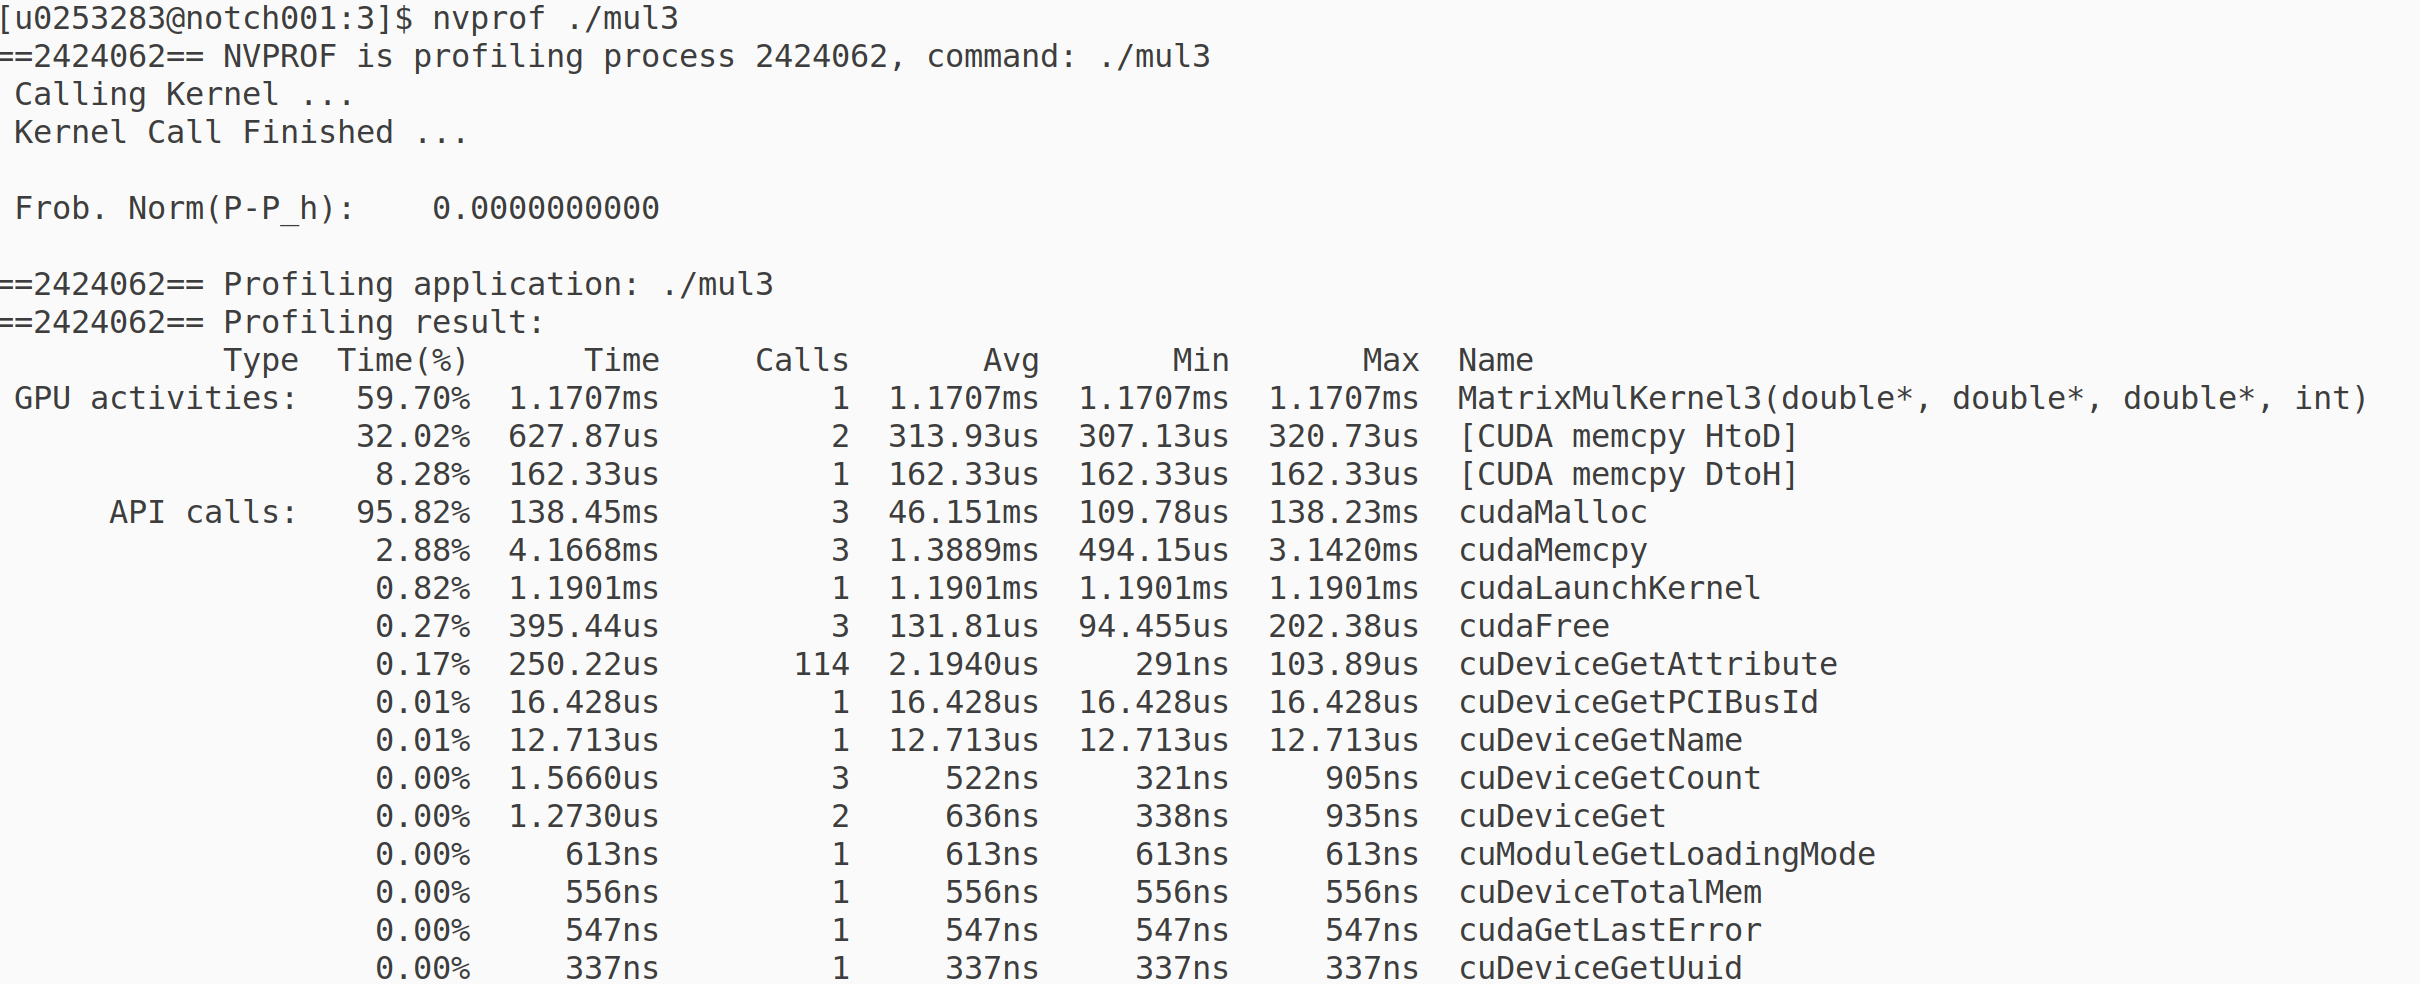
\includegraphics[width=0.95\textwidth]{./img/nvprof-mul3.png}
          \caption{\small{Profiling \texttt{mul3} on \texttt{notch001}}}
     \end{figure}
     \end{columns}
\end{frame}	


% CUDA Libraries: CUBLAS, CUFFT, CUDNN, MAGMA, CURAND, NCCL
\subsection{Important CUDA libraries}
\begin{frame}
   \frametitle{Important CUDA libraries}
     In order to increase the performance of your code we recommend 
     to use highly-optimized libraries. Among them, we have:
     \begin{itemize}
	\item \href{https://developer.nvidia.com/cublas}{\textbf{\textcolor{green}{cuBLAS}}}: 
		\textbf{B}asic \textbf{L}inear \textbf{A}lgebra \textbf{S}ubroutines on NVIDIA GPUs.
	\item \href{https://icl.utk.edu/magma/}{\textbf{\textcolor{green}{MAGMA}}}: 
		\textbf{M}atrix \textbf{A}lgebra on \textbf{G}PU and \textbf{M}ulti-core \textbf{A}rchitectures. 		
        \item \href{https://docs.nvidia.com/cuda/pdf/CURAND_Library.pdf}{\textbf{\textcolor{green}{cuRAND}}}: Random Number Generation library.
        \item \href{https://docs.nvidia.com/cuda/pdf/CUFFT_Library.pdf}{\textbf{\textcolor{green}{cuFFT}}}: 
		CUDA \textbf{F}ast \textbf{F}ourier \textbf{T}ransform library.
	\item \href{https://developer.nvidia.com/nccl}{\textbf{\textcolor{green}{NCCL}}}: 
	  \textbf{N}VIDIA \textbf{C}ollective \textbf{C}ommunications \textbf{L}ibrary. 		
	\item \href{https://developer.nvidia.com/cudnn}{\textbf{\textcolor{green}{cuDNN}}}: 
  	  CUDA \textbf{D}eep \textbf{N}eural \textbf{N}etwork library.		
	\item \href{https://developer.nvidia.com/cutensor}{\textbf{\textcolor{green}{cuTENSOR}}}: GPU-accelerated Tensor Linear Algebra.
	\item \href{https://developer.nvidia.com/DALI}{\textbf{\textcolor{green}{DALI}}}: Library for decoding \& augmenting images (DL applications).
        \item $\ldots$
     \end{itemize}
\end{frame}


% Alternatives:
%  - Within CUDA: CudaFortran, OpenAcc (pragmas)
%  - Alternatives to CUDA: OpenCL, HIP
%  - Kokkos
\subsection{Alternatives to CUDA}
\begin{frame}
   \frametitle{Alternatives to CUDA}
      \begin{itemize}
         \item Similar to CUDA
   	    \begin{itemize}
	       \item \href{https://www.amd.com/en/products/software/rocm.html}{\textbf{\textcolor{green}{ROCM}}} (AMD)
  	    \end{itemize} 
          \item \href{https://www.openacc.org/}{\textbf{\textcolor{green}{OpenACC}}} (use of directives (cfr. \texttt{OpenMP})
             \begin{itemize}
                \item GCC: supports OpenACC for NVIDIA  \& AMD GPUs. 
                \item NVIDIA HPC SDK (formerly PGI)
                \item Sourcery Codebench (AMD GPU) % https://www.openacc.org/tools/sourcery-codebench 			
	     \end{itemize}
          \item Higher-level abstractions
             \begin{itemize}
		\item \href{https://www.kokkos.org/about/core/}{\textbf{\textcolor{green}{Kokkos}}} (prog. model for parallel algorithms for many-core chips)
             \end{itemize}
      \end{itemize}
\end{frame}	

\subsection{Links}
\begin{frame}
   \frametitle{Links}
      \begin{itemize}
         \item \href{https://docs.nvidia.com/cuda/index.html}{CUDA Toolkit Documentation}
	 \item \href{https://docs.nvidia.com/cuda/cuda-c-programming-guide/index.html}{CUDA \CC\, Programming Guide Release $12.6$ 
		 (10/01/24)}
	 \item \href{https://docs.nvidia.com/cuda/cuda-c-best-practices-guide/index.html}{CUDA \CC\, Best Practices Guide, Release $12.6$ (09/24/24)}	      
         \item \href{https://docs.nvidia.com/cuda/cuda-compiler-driver-nvcc/}{NVIDIA CUDA Compiler Driver NVCC, Release $12.6$ (09/24/24)}		 
         \item \href{https://docs.nvidia.com/cuda/parallel-thread-execution/}{PTX \& ISA Release $8.5$ (09/24/24)}	
		 
      \end{itemize}		      
\end{frame}	


\section{Use of GPUs at the CHPC}

\subsection{GPUs available at CHPC}

\subsubsection{lp/kp/np/grn}
\begin{frame}
        \frametitle{GPU devices on lp/kp/np/grn}
\begin{table}[H]
   \begin{center}
     \begin{tabular}{c|c}
        \multirow{2}{*}{\texttt{GPU device type}} & \texttt{compute} \\
                                                 & \texttt{capability} \\
        \hline
	  \href{https://www.nvidia.com/en-us/geforce/graphics-cards/geforce-gtx-titan-x/specifications/}{\small{\texttt{NVIDIA GeForce GTX TITAN X}}} & \small{5.2} \\
	  \href{https://images.nvidia.com/content/tesla/pdf/nvidia-tesla-p100-PCIe-datasheet.pdf}{\small{\texttt{Tesla P100-PCIE-16GB}}} & \small{6.0} \\
	  \href{https://www.nvidia.com/content/dam/en-zz/Solutions/design-visualization/documents/nvidia-p40-datasheet.pdf}{\small{\texttt{Tesla P40}}}& \small{6.1} \\
	  \href{https://www.nvidia.com/en-us/geforce/10-series/\#1080-ti-spec}{\small{\texttt{NVIDIA GeForce GTX 1080 Ti}}}    &  \small{6.1}  \\
	  \href{https://www.gpuzoo.com/GPU-NVIDIA/Titan\_V.html}{\small{\texttt{NVIDIA Titan V}}} & \small{7.0} \\  
	  \href{https://images.nvidia.com/content/technologies/volta/pdf/tesla-volta-v100-datasheet-letter-fnl-web.pdf}{\small{\texttt{NVIDIA Tesla V100-PCIE-16GB}}} & \small{7.0} \\
	  \href{https://www.nvidia.com/content/dam/en-zz/Solutions/Data-Center/tesla-t4/t4-tensor-core-product-brief.pdf}{\small{\texttt{Tesla T4}}} & \small{7.5} \\
	  \href{https://www.techpowerup.com/gpu-specs/geforce-rtx-2080-ti.c3305}{\small{\texttt{NVIDIA GeForce RTX 2080 Ti}}} & \small{7.5} \\   
	  \href{https://www.nvidia.com/content/dam/en-zz/Solutions/Data-Center/a100/pdf/nvidia-a100-datasheet-us-nvidia-1758950-r4-web.pdf}{\small{\texttt{NVIDIA A100-PCIe-40GB}}} & \small{8.0} \\
	  \href{https://www.nvidia.com/content/dam/en-zz/Solutions/Data-Center/a100/pdf/nvidia-a100-datasheet-us-nvidia-1758950-r4-web.pdf}{\small{\texttt{NVIDIA A100-SXM4-80GB}}} & \small{8.0} \\
	  \href{https://www.nvidia.com/en-us/design-visualization/a800/}{\small{\texttt{NVIDIA A800 40GB Active}}} & \small{8.0}  \\
        \hline
    \end{tabular}
   \end{center} 
   \caption{GPU devices on lp/kp/np/grn (10/01/2024)}
\end{table}
\end{frame} 

\begin{frame}
	\frametitle{GPU devices on lp/kp/np/grn (cont.)}
\begin{table}[H]
   \begin{center}
     \begin{tabular}{c|c}
         \multirow{2}{*}{\texttt{GPU device type}} & \texttt{compute} \\
                                                 & \texttt{capability} \\
      \hline
        \href{https://www.nvidia.com/en-us/geforce/graphics-cards/30-series/rtx-3090-3090ti/}{\small{\texttt{NVIDIA GeForce RTX 3090}}} & \small{8.6} \\ 
        \href{https://images.nvidia.com/content/Solutions/data-center/a40/nvidia-a40-datasheet.pdf}{\small{\texttt{NVIDIA A40}}}     & \small{8.6} \\
	     \href{https://www.nvidia.com/content/dam/en-zz/Solutions/gtcs22/design-visualization/quadro-product-literature/proviz-nvidia-rtx-a5500-datasheet-2130578-r3-us-web.pdf}{\small{\texttt{NVIDIA RTX A5500}}} & \small{8.6} \\
	     \href{https://www.nvidia.com/en-us/design-visualization/rtx-a6000/}{\small{\texttt{NVIDIA RTX A6000}}} & \small{8.6} \\
	     \href{https://www.nvidia.com/content/dam/en-zz/Solutions/design-visualization/rtx-6000/proviz-print-rtx6000-datasheet-web-2504660.pdf}{\small{\texttt{NVIDIA RTX 6000 Ada Generation}}}&  \small{8.9} \\
	     \href{https://www.nvidia.com/en-us/data-center/l40/}{\small{\texttt{NVIDIA L40}}} & \small{8.9} \\
	     \href{https://resources.nvidia.com/en-us-l40s/l40s-datasheet-28413}{\small{\texttt{NVIDIA L40S}}} & \small{8.9} \\
	     \href{https://www.nvidia.com/en-us/data-center/h100/}{\small{\texttt{NVIDIA H100 NVL}}}/\href{https://www.nvidia.com/content/dam/en-zz/Solutions/Data-Center/h100/PB-11773-001\_v01.pdf}{\small{\texttt{Deep Dive}}} &  \small{9.0} \\
        \hline
     \end{tabular}
   \end{center}
   \caption{GPU devices on lp/kp/np/grn (10/01/2024)}
\end{table}
\end{frame}

\subsubsection{redwood}
\begin{frame}
	\frametitle{GPU devices on redwood}	
\begin{table}[H]
   \begin{center}
     \begin{tabular}{c|c}
       \multirow{2}{*}{\texttt{GPU device type}} & \texttt{compute} \\
                                                 & \texttt{capability} \\
       \hline
       \href{https://www.nvidia.com/en-us/geforce/10-series/\#1080-ti-spec}{\small{\texttt{NVIDIA GeForce GTX 1080 Ti}}}    &  \small{6.1}  \\
       \href{https://www.nvidia.com/content/dam/en-zz/Solutions/Data-Center/a100/pdf/nvidia-a100-datasheet-us-nvidia-1758950-r4-web.pdf}{\small{\texttt{NVIDIA A100-SXM4-40GB}}} &  \small{8.0} \\
	     \href{https://www.nvidia.com/content/dam/en-zz/Solutions/Data-Center/a100/pdf/nvidia-a100-datasheet-us-nvidia-1758950-r4-web.pdf}{\small{\texttt{NVIDIA A100 80GB PCIe}}} &  \small{8.0} \\
	     \href{https://www.nvidia.com/content/dam/en-zz/Solutions/data-center/products/a30-gpu/pdf/a30-datasheet.pdf}{\small{\texttt{NVIDIA A30}}}   &  \small{8.0} \\
	     \href{https://images.nvidia.com/content/Solutions/data-center/a40/nvidia-a40-datasheet.pdf}{\small{\texttt{NVIDIA A40}}} &  \small{8.6} \\
	     \href{https://www.nvidia.com/content/dam/en-zz/Solutions/design-visualization/rtx-6000/proviz-print-rtx6000-datasheet-web-2504660.pdf}{\small{\texttt{NVIDIA RTX 6000 Ada Generation}}}&  \small{8.9} \\
	     \href{https://www.nvidia.com/en-us/data-center/h100/}{\texttt{NVIDIA H100 NVL}}/\href{https://www.nvidia.com/content/dam/en-zz/Solutions/Data-Center/h100/PB-11773-001\_v01.pdf}{\small{\texttt{Deep Dive}}} &  \small{9.0} \\
        \hline
     \end{tabular}
   \end{center}	   
   \caption{GPU devices on redwood (10/01/2024)}
\end{table}	   
\end{frame}	
          % Use of GPUs at the CHPC

% --- END ---
\section*{Questions}
\begin{frame}
   \frametitle{Questions?}
   Thank you!\newline	
   Any questions?
\end{frame}
      % Questions

\end{document}          % End Document
